\newcommand{\addREf}{\todo{REF HERE}}

\subsection{\softner{} Deep Learning Model}
\label{sec:multi-task-model}
The previous sections explain the phases of the \softner{} framework, as shown in Figure \ref{fig:overview}, that automate the significant task of creating labeled data for deep learning models which can further generalize knowledge extraction. Here we propose a novel Multi Task deep learning model that solves two entity recognition tasks simultaneously, i.e., Entity Type recognition and Data Type recognition.

The model uses an architecture, as described in Figure \ref{model-arch}, that shares some common parameters and layers for both tasks, but also has task specific layers. Incident descriptions are converted to word level vectors using a pre-trained Glove Embedding layer. This sequence of vectors is interpreted, both forwards and in reverse, by a Bi-directional LSTM layer. We then have distinct layers for the two tasks. The time-distributed layer transposes the BiLSTM hidden vectors to the shape of the output labels and the attention mechanism helps the model bias it's learning towards important sections of the sentences. Finally, the CRF layer produces a valid sequence of output labels. We perform back propagation using a combination of loss functions during training and evaluate individual tag precision, recall and F1 metrics. In the following sub sections we describe the important layers and approaches used in our multi task model.

\subsubsection{\textbf{Word Embeddings}}
\label{sec:glove-word-emb}
Language models in the semantic vector space, require real valued vectors as word representations. The importance of these vectors in improving performance for NLP tasks has been widely studied \cite{collobert2011natural}. These vectors act as characteristic features in applications of language models like question answering, document classification and named entity recognition.
GloVe \cite{pennington2014glove}, introduced a model that captures linear substructure relations in a global corpus of words, revealing regularities in syntax as well as semantics. The GloVe model trained on 5 different corpora, covers a vast range of topics and tokens. GloVe vectors, demonstrated on tasks such as word analogy and named entity recognition in \cite{pennington2014glove}, outperforms various other word representations. To use the 100 dimension version of GloVe, we create an embedding layer with the pre-trained GloVe weights in all our models.

\subsubsection{\textbf{Bi-directional LSTM}}
Recurrent Neural Networks (RNN) have been the basis for numerous language modelling tasks in the past.\cite{mikolov2010recurrent}. An RNN maintains historic information extracted from sequence or series like data. This feature enables RNN based models to make predictions at a certain time step, conditional to the viewed history. They take a sequence of vectors $\boldsymbol{(x_1, x_2, .., x_n)}$ as input and return a sequence of vectors $\boldsymbol{(h_1, h_2, .., h_3)}$ that encodes information at every time step.
Although it can be hypothesized that RNNs are capable of encoding and learning dependencies that are spread over long time steps, evidence shows that they fail to do so. RNNs tend to be biased towards more recent updates in long sequence situations.

Long Short-term Memory (LSTM) networks \cite{hochreiter1997long} were designed to overcome the problems associated with vanilla RNNs. Their architecture allows them to capture long range dependencies using several gates. These gates control the portion of the input to give to the memory cell, and the portion from the previous hidden state to forget. We model the LSTM layer using the following equations:
%
\begin{equation}
    f_{t}=\sigma(W_{f}\cdot[h_{t-1},x_{t}] + b_{f})
\end{equation}
\begin{equation}
    i_{t}=\sigma(W_{i}\cdot[h_{t-1},x_{t}] + b_{i})
\end{equation}
\begin{equation}
    {\tilde {c}}_{t}=\tanh(W_{c}\cdot[h_{t-1},x_{t}] + b_{c})
\end{equation}
\begin{equation}
    c_{t}= f_{t}\circ c_{t-1}+ i_{t}\circ {\tilde {c}}_{t}
\end{equation}
\begin{equation}
    o_{t}=\sigma(W_{o}\cdot[h_{t-1},x_{t}] + b_{o})
\end{equation}
\begin{equation}
    h_{t}=o_{t}\circ \tanh(c_{t})
\end{equation}

In the above equations $\sigma$ is the element wise sigmoid function and the $\circ$ represents hadamard product (element-wise). $f_t, i_t$ and $o_t$ are forget, input, and output gate vectors respectively, and, $c_t$ is the cell state vector. Using the above equations, given a sentence as a sequence of real valued vectors $\boldsymbol{(x_1, x_2, .., x_n)}$, it computes $\overrightarrow{h_{t}}$ that represents the leftward context of the word at the current time step $t$. By intuition, a word at the current time step $t$, receives context from other words that occur on either sides. A representation of this can be achieved with a second LSTM that interprets the same sequence in reverse, returning $\overleftarrow{h_{t}}$ at each time step. This combination of forward and backward LSTM is referred to as Bi-Directional LSTM (BiLSTM) \cite{graves2005framewise}. The final representation of the word is produced by concatenating the left and right context, $h_{t}=[\overrightarrow{h_{t}};\overleftarrow{h_{t}}]$.


\subsubsection{\textbf{Neural Attention Mechanism}}
In recent years attention mechanism has become increasing popular in various NLP applications like neural machine translation \cite{bahdanau2014neural}, sentiment classification \cite{chen2017recurrent} and parsing \cite{li2016discourse}. Novel architectures like transformers \cite{vaswani2017attention} and BERT \cite{devlin2018bert} have proven the effectiveness of such a mechanism for various downstream tasks. In addition to the improvements BiLSTMs bring to the original RNN approach, attention mechanism addresses long input sequences by retaining and utilising all hidden states generated. We implement attention at the word level as a neural layer, with a weight parameter $W_{a}$. It takes as input the the hidden states from the BiLSTM, transposed to output dimensions using a time distributed dense layer. Let $h = [h_1, h_2, .. h_{T}]$ be the input to the attention layer. The attention weights and final representation $h^*$ of the sentence is formed as follows:
\begin{equation}
    scores = W_a^Th
\end{equation}
\begin{equation}\label{attention-score}
    \alpha = softmax(scores)      
\end{equation}
\begin{equation}
    r = h\alpha^T    
\end{equation}
\begin{equation}\label{attention-repr}
    h^* = \tanh(r)    
\end{equation}

In equations \ref{attention-score} \& \ref{attention-repr} the $softmax$ and $tanh$ functions are applied element-wise on the input vectors. We then concatenate $h$ and $h^*$ and pass it to the next layer. We visualize the attention vector $\alpha$ for a test sentence in Figure \ref{attention-viz}, where we observe that the attention layer learns to give more emphasis to tokens that have a higher likelihood of being entities. In Figure \ref{attention-viz}, the darkness in the shade of blue is proportional to the degree of attention. In case of long sequences, this weighted attention to certain sections of the sequence, that are more likely to contain entities, helps improve the model's sensitivity\footnote{Sensitivity, also known as recall, is the proportion of actual positives that are correctly identified}.

\begin{figure}%[H]
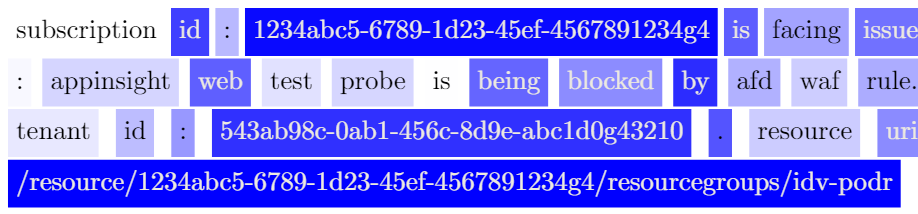
\includegraphics[width=\linewidth]{Figures/attention_viz.png}
\vspace{-12pt}
\caption{Attention visualization on a sample input}
\label{attention-viz}
\vspace{-6pt}
\end{figure}

\subsubsection{\textbf{Conditional Random Fields}}
A simple approach to sequence tagging with LSTMs is to use the hidden state representations ($h_t$) as word features to make independent tagging decisions at the word level. But that leaves behind inherent dependencies across output labels in tasks like Named Entity Recognition. Our NER task also has this characteristic since the initial \softner{} heuristics enforce structural constraints, for example, separators between key-value and html table tags. In learning these dependencies and generalizing them to sentences without these constraints, we model tagging decisions jointly using conditional random fields 
\cite{lafferty2001conditional}.

For an input sequence $\boldsymbol{X = (x_1, x_2, .., x_n)}$, let $\boldsymbol{y = (y_1, y_2, .., y_n)}$ a potential output sequence, where n is the no of words in the sentence. Let $P$, the output of the BiLSTM network passed through the dense and attention layers, be the matrix of probability scores of shape $n \times k$, where k is the number of distinct tags. That is $P_{i,j}$ is a score that the $i^{th}$ word corresponds to the $j^{th}$ tag. We define CRF as a layer in the model, whose working is as follows. First a score is computed for $y$.

\begin{equation}
    s(\boldsymbol{X,y}) = \sum_{i=0}^{n} A_{y_i,y_{i+1}} + \sum_{i=0}^{n} P_{i,y_{i}} 
\end{equation}

where A represents the matrix of transition scores. That is $A_{i,j}$ is the score for the transition from $tag_i$ to $tag_j$. Then the score is converted to a probability for the sequence $y$ to be the right output using a softmax over $\boldsymbol{Y}$(all possible output sequences). 

\begin{equation}
    p(\boldsymbol{y|X}) = 
    \dfrac{e^{s(\boldsymbol{X,y})}}{\sum_{y' \in Y} e^{s(\boldsymbol{X,y'})}  }
\end{equation}

The model learns by maximizing the log-probability of the correct $y$. While extracting the tags for the input, we predict the output sequence with the highest score.

\begin{equation}
    \boldsymbol{y^*} = \argmax_{y' \in Y} p(y'|X)
\end{equation}

From the above implementation it is clear as to how the CRF and attention layers push the model towards learning a valid sequence of tags, unlike in the case of independent tagging as discussed.

\begin{figure}%[H]
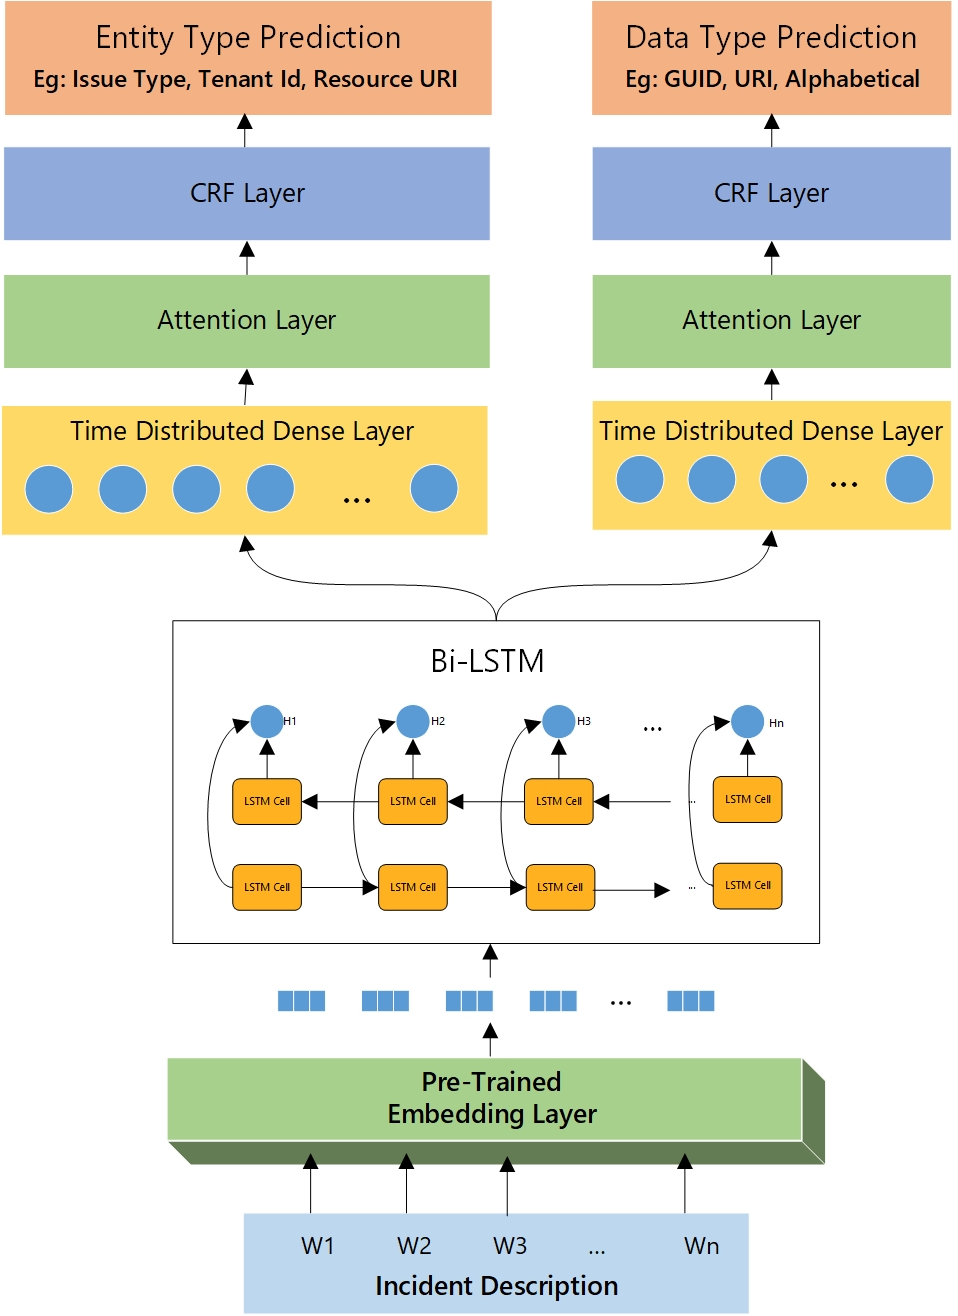
\includegraphics[width=\linewidth]{Figures/MTL_Diagram.jpg}
\caption{Multi-task model architecture}
\label{model-arch}
%\vspace{-6pt}
\end{figure}

\subsubsection{\textbf{Multi-Task Learning}}

Caruana et al. \cite{caruana1997multitask} defines Multi-Task Learning (MTL) as an approach to improve generalization in models by using the underlying common information contained among related tasks. Some well known applications for MTL are multi-class and multi-label classification problems. In the context of classification or sequence labelling, MTL improves the performance of individual tasks by learning them jointly.

In \softner{}, named-entity recognition is the primary task. In this task, models mainly learn from context words that support occurrences of entities. But we also observe that incorporating a complimentary task of predicting the data-type of a token reinforces intuitive constraints, indirectly to model training. For example in an input like "\textit{The SourceIPAddress is 127.0.0.1}", the token \textit{127.0.0.1} is identified more accurately by our model, as the entity type "\textbf{Source Ip Address}", because it is also identified as the data-type "\textbf{Ip Address}", in parallel. This supplements the intuition that all \textit{Source Ip Addresses} are \textit{Ip adresses}, thus, improving model performance. Therefore, we choose data type prediction as the auxiliary task for \softner{}'s deep learning model.

There are multiple architectures that allow multi-task learning, like Multi-head architecture, Cross-snitch Networks\cite{misra2016cross} and Sluice Networks \cite{ruder2017learning}. We use the Multi-head architecture, where the lower level features generated by the BiLSTM layers are shared, whereas the other layers are task specific. The combined architecture is depicted in Figure \ref{model-arch}. As stated above, we define the entity type prediction as the main task and that of data type prediction as the auxiliary task. The losses are initially calculated individually for both tasks, $l_1$ and $l_2$, and then combined into $loss_{c}$ using a weighted sum. The parameter $loss\_weights = (\alpha,\beta)$ is used to control the importance between main and auxiliary task as follows:

\begin{equation}
    loss_{c} = \alpha \times l_1 + \beta \times l_2
\end{equation}

During training, the model aims to minimize the $loss_{c}$ but the individual losses are back-propagated to only those layers that produced the output. With such an approach, the lower level common layers are trained by both tasks, whereas the task specific layers are trained by individual losses.